\documentclass{beamer}

\usepackage[utf8]{inputenc}
\usepackage[english]{babel}
\usepackage{textpos}
\usepackage{graphicx}
\usepackage{textcomp}
\usepackage{animate}
\usepackage{comment}
%\usepackage{multicol}
%\setlength{\columnsep}{5cm}
\usepackage{amsmath}
\usepackage{amsfonts}
\usepackage{verbatim}
\usepackage{varwidth}
\usepackage{caption}
\usepackage{dcolumn}
\usepackage{amssymb}
\usepackage{algorithm}
\usepackage{algorithmic}
%\usepackage{physics}
\usepackage{hyperref}
\usepackage{scalerel,stackengine}
%\usepackage{fancyvrb}


\newcommand{\code}[1]{\texttt{#1}}
\newcommand{\shp}{$>>>$ }
\newcommand{\tab}{\hspace*{22pt}}

\usetheme{Madrid}

\title{Chapter 7 pt 1: \\ Reading and Writing Files}
\author{EEC 3150}
\date{}

\institute{Trevecca Nazarene University}
 


%%%%%%%%% BEGIN DOCUMENT %%%%%%%%%
%%%%%%%%% BEGIN DOCUMENT %%%%%%%%%
%%%%%%%%% BEGIN DOCUMENT %%%%%%%%%

\begin{document}

% get title page 
\frame{\titlepage}
 
%%%%%%%%%%
%%%%%%%%%%
\begin{frame}	
	\frametitle{Outline}
	\tableofcontents	
\end{frame}


%%%%%%%%%%
%%%%%%%%%%
\section{Basic of Reading Files}

\begin{frame}	
	\center{\Huge{Basic of Reading Files}}
\end{frame}

\begin{frame}	
	\frametitle{Basic of Reading Files}
	
	\begin{block}{Intro to reading a file with Python:}
		\minipage{0.5\textwidth}
			\code{fname = "FirstFile.txt" \\
					\tab \\
					fhandle = open(fname, 'r')  \\
					\tab \\
					string = fhandle.read() \\
					print(string) \\
					\tab \\
					fhandle.close() 
			}
		\endminipage\hfill
		\minipage{0.5\textwidth}
			\begin{itemize}
				\item To read a file, use the \code{open()} function
				\item Two string arguments: 1) the filename, 2) whether to read (`r'), write (`w'), or append (`a') to the file
				\item Returns a \emph{file handle} (essentially a variable that points to the file)
				\item Since file handles are objects, the have their own methods (such as \code{read()})
				\item Close the file when finished
				\item Trying to read after closing throws an error
			\end{itemize}
		\endminipage\hfill
	\end{block}
	
\end{frame}

\begin{frame}	
	\frametitle{Basic of Reading Files}
	
	\begin{block}{Reading files in a \code{with,as} block:}
		\minipage{0.6\textwidth}
			\begin{itemize}
				\item Closing a file is annoying and you can forget to do it
				\item For convenience, we can read files inside a \code{with,as} block
			\end{itemize}
			
			\vspace{20pt}
			\code{fname = "FirstFile.txt" \\
					with open(fname, 'r') as fhandle:
					\tab string = fhandle.read() \\
					\tab print(string)
			}
		\endminipage\hfill
		\minipage{0.4\textwidth}
			\begin{itemize}
				\item The file handle is only defined in the scope of the block
				\item Variables you define inside the block will still be defined after the block
				\item The file is closed automatically after the block is finished
				\item Read the file in the block, save the contents to a variable, and use them later on
			\end{itemize}
		\endminipage\hfill
	\end{block}
	
\end{frame}

\begin{frame}	
	\frametitle{Basic of Reading Files}
	
	\begin{block}{Some read methods:}
		\minipage{0.6\textwidth}
			\vspace{10pt}
			
			\code{with open(fname, 'r') as fhandle:
					\tab string = fhandle.read() \\
			}
			
			\vspace{10pt}
			\code{with open(fname, 'r') as fhandle:
					\tab lines = fhandle.readlines() \\
			}
		\endminipage\hfill
		\minipage{0.05\textwidth}
		\endminipage\hfill
		\minipage{0.35\textwidth}
			\code{fhandle.read()}
			\begin{itemize}
				\item Returns the entire file in one string
			\end{itemize}
			
			\vspace{10pt}
			\code{fhandle.readlines()}
			\begin{itemize}
				\item Returns a list of strings split on newlines
			\end{itemize}
		\endminipage\hfill
	\end{block}
	
\end{frame}

\begin{frame}	
	\frametitle{Basic of Reading Files}
	
	\begin{block}{Reading a line at a time:}
		\minipage{0.6\textwidth}
			\vspace{30pt}
			
			\code{with open(fname, 'r') as fhandle:
					\tab for line in fhandle: \\
					\tab \tab print(line)
			}
			
			\vspace{30pt}
			\code{with open(fname, 'r') as fhandle:
					\tab line = fhandle.readline() \\
					\tab print(line) \\
					\tab line = fhandle.readline() \\
					\tab print(line)
			}
		\endminipage\hfill
		\minipage{0.05\textwidth}
		\endminipage\hfill
		\minipage{0.35\textwidth}
			With a for loop:
			\begin{itemize}
				\item We can read a line at a time with a for loop
			\end{itemize}
			
			\vspace{20pt}
			\code{fhandle.readline()}
			\begin{itemize}
				\item Returns the next line
			\end{itemize}
		\endminipage\hfill
	\end{block}
	
\end{frame}

\begin{frame}	
	\frametitle{Basic of Reading Files}
	
	\begin{block}{Reading a line at a time:}
		\minipage{0.6\textwidth}
%			\vspace{30pt}		
			\code{with open(fname, 'r') as fhandle:
					\tab line = fhandle.readline() \\
					\tab while line: \\
					\tab \tab print(line) \\
					\tab \tab line = fhandle.readline()
			}
		\endminipage\hfill
		\minipage{0.05\textwidth}
		\endminipage\hfill
		\minipage{0.35\textwidth}
			With a while loop:
			\begin{itemize}
				\item We can read a line at a time with a while loop
				\item Read the first line
				\item Use the line as the loop condition
				\item Once \code{readline()} returns an empty string, the loop exits
			\end{itemize}
		\endminipage\hfill
	\end{block}
	
\end{frame}

\begin{frame}	
	\frametitle{Basic of Reading Files}
	
	\begin{block}{Filepaths:}
		\begin{itemize}
			\item Unless specified, Python assumes that the file you want to read/write is in the same folder/directory as the script
			\item If it isn't, you must provide a \emph{filepath} for the file (its location on your computer's hard drive)
		\end{itemize}
		Two kinds of filepaths (say our script is in the \code{Python} directory):
		\begin{itemize}
			\item \textbf{Absolute}: a filepath from the root directory of the drive to the file: \\
			Ex: \code{C:/Users/Graham West/Python/Data/FirstFile.txt}
			\item \textbf{Relative}: a filepath from the script directory to the file: \\
			Ex: \code{Data/FirstFile.txt}
		\end{itemize}
	\end{block}
	
\end{frame}

\begin{frame}	
	\frametitle{Basic of Reading Files}
	
	\begin{block}{Parent directory command: ..}
		\minipage{0.5\textwidth}
			\begin{figure}[ht]
				\centering
				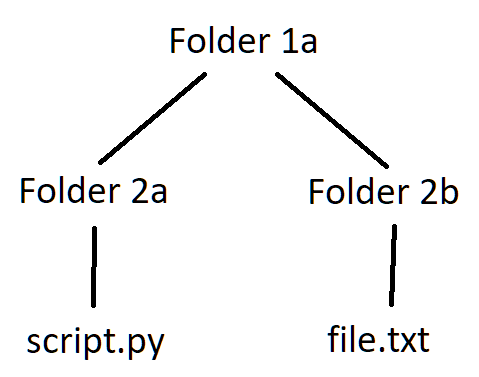
\includegraphics[width=\linewidth]{ParentDirectory}
			\end{figure}
		\endminipage\hfill
		\minipage{0.5\textwidth}
			\begin{itemize}
				\item If you need to navigate to the parent directory, you can include ``..'' in your relative filepath: \\
				Ex: \code{../Folder 2b/file.txt}
			\end{itemize}
		\endminipage\hfill
	\end{block}
	
\end{frame}


%%%%%%%%%%
%%%%%%%%%%
\section{Extracting Data from Files}

\begin{frame}	
	\center{\Huge{Extracting Data from Files}}
\end{frame}

\begin{frame}	
	\frametitle{Extracting Data from Files}
	
	\begin{exampleblock}{Get a list of grades from a file:}
		Read the file Grades.txt and produce a list of integer grades.
		\begin{itemize}
			\item This file is simple and has one number per line
		\end{itemize}
	\end{exampleblock}
	
	\begin{exampleblock}{Get lists of years and temperatures from a file:}
		Read the file YearTemp.txt and produce lists of integer years and float temperatures.
		\begin{itemize}
			\item This file is more complicated
			\item It has a header that we must ignore
			\item Year and temp values are comma-separated (one pair per line)
		\end{itemize}
	\end{exampleblock}
	
\end{frame}

\begin{frame}	
	\frametitle{Extracting Data from Files}
	
	\begin{exampleblock}{Get 2D list galaxy simulation parameters:}
		Read the file \code{587722984435351614\_combined.txt} and produce a2D list of simulation parameters and a 1D list of simulation fitnesses.
		\begin{itemize}
			\item File has no header
			\item Each line has two comma-separate sections which have a tab n/t them
			\item At a certain line number, the are no more fitness values, so stop reading here
		\end{itemize}
	\end{exampleblock}
	
\end{frame}

\begin{frame}	
	\frametitle{Extracting Data from Files}
	
	\begin{exampleblock}{Get electron density parameters from files:}
		Write a program that can read any of the following files (\code{h2o.txt, nh3.txt, ch4.txt}) and create lists of the \code{CENTRE ASSIGNMENTS} (note the spelling), \code{TYPE ASSIGNMENTS}, and \code{EXPONENTS}.
		\begin{itemize}
			\item The values span multiple lines
			\item Each file spans a different number of lines
			\item The program should be able to handle all possible cases
		\end{itemize}		
	\end{exampleblock}
	
\end{frame}


%%%%%%%%%%
%%%%%%%%%%
\section{Writing to Files}

\begin{frame}	
	\center{\Huge{Writing to Files}}
\end{frame}

\begin{frame}	
	\frametitle{Writing to Files}
	
	\begin{block}{Writing files in a \code{with,as} block:}
		\minipage{0.5\textwidth}
			\code{fname = "Write.txt" \\
					with open(fname, 'w') as f:
					\tab f.write(`test')
			}
		\endminipage\hfill
		\minipage{0.5\textwidth}
			\begin{itemize}
				\item Open the file in the same as before, but now with \code{`w'}
				\item Use the \code{write()} function
			\end{itemize}
		\endminipage\hfill
	\end{block}
	
	\begin{block}{The \code{writelines()} function:}
		\minipage{0.5\textwidth}
			\code{fname = "Write.txt" \\
					with open(fname, 'w') as f:
					\tab x = [`1\textbackslash n', `2\textbackslash n'] \\
					\tab f.writelines(x)
			}
		\endminipage\hfill
		\minipage{0.5\textwidth}
			\begin{itemize}
				\item The \code{writelines()} function can accept a list of strings and write all of them to a file
				\item HOWEVER, despite its name, it doesn't automatically add newlines (\textbackslash n) at the end of each string in the list; you must do it manually
			\end{itemize}
		\endminipage\hfill
	\end{block}
	
\end{frame}

\begin{frame}	
	\frametitle{Writing to Files}
	
	\begin{exampleblock}{Write a csv file:}
		Write a program that will write a 2D list of numbers to a file. The numbers on each line should be comma-separated.
	\end{exampleblock}
	
\end{frame}


%%%%%%%%%%
%%%%%%%%%%
\section{Formatting Strings}

\begin{frame}	
	\center{\Huge{Formatting Strings}}
\end{frame}

\begin{frame}	
	\frametitle{Formatting Strings}
	
	\begin{block}{The \code{str.format()} method:}
		The \code{str.format()} method lets you manually format string in various ways:
		
		\vspace{10pt}
		\code{"My name is \{fname\}, I'm \{age\}".format(name="John",age=36)\\
		"My name is \{0\}, I'm \{1\}".format("John",36)\\
		"My name is \{\}, I'm \{\}".format("John",36) \\[10pt]
		My name is John, I'm 36
		}
		
		\vspace{10pt}
		\begin{itemize}
			\item Call the method with the string you want to format
			\item Insert args of function into the string with curly brackets: \{\}
			\item The args can be inserted via keywords, numbers, or in order of appearance (by default, last example above)
		\end{itemize}
	\end{block}
	
\end{frame}

\begin{frame}	
	\frametitle{Formatting Strings}
	
	\begin{block}{Padding strings:}
		The real power of \code{str.format()} lies in \emph{padding} (insertion of whitespace for readability):
		\begin{itemize}
			\item \code{``\{:10\}''.format(``test'')} \\
					This will return string that is 10 characters long and starts with ``test'' (extra characters are spaces)
			\item \code{``\{:$>$10\}''.format(``test'')} \\
					This will return string that is 10 characters long and ends with ``test'' (extra characters are spaces)
		\end{itemize}
		Why do we care?
		\begin{itemize}
			\item If we wants to print/write multiples of different length, we can pad them so that they are aligned
		\end{itemize}
	\end{block}
	
\end{frame}

\begin{frame}	
	\frametitle{Formatting Strings}
	
	\begin{block}{Padding with floats:}
		Padding is very useful when dealing with floating point numbers with different numbers of decimals:
		\begin{itemize}
			\item \code{``\{:$m$.$n$f\}''.format(number)} \\
					$m$: the total number of characters (the length) \\
					$n$: the number of decimal places (padded with zeroes)
			\item \code{``\{:10.4f\}''.format(100.01)}
			\item To assign these numbers from variables, simply add more curly brace pairs: \\
					\code{``\{:\{\}.\{\}f\}''.format(100.01,10,4)}
			\item If this is confusing, add the argument indices: \\
					\code{``\{0:\{1\}.\{2\}f\}''.format(100.01,10,4)}
		\end{itemize}
	\end{block}
	
\end{frame}

\begin{frame}	
	\frametitle{Writing to Files}
	
	\begin{exampleblock}{Write formatted numbers to a file:}
		Write a program that will
		\begin{itemize}
			\item write a list of floats to a file
			\item in a right justified fashion
			\item with all decimals aligned
			\item with a consistent number of decimals
			\item by passing the length and number of decimals as an argument to \code{format()}
			\item and determine the minimum value of these numbers from the list
		\end{itemize}
	\end{exampleblock}
	
\end{frame}


%%%%%%%%%%
%%%%%%%%%%
\section{Formatting Strings}

\begin{frame}	
	\center{\Huge{Appending to Files}}
\end{frame}

\begin{frame}	
	\frametitle{Appending to Files}
	
	\begin{block}{Opening a file in append mode: `a'}
		\minipage{0.5\textwidth}
			\code{fname = "Write.txt" \\
					with open(fname, 'a') as f:
					\tab x = [`1\textbackslash n', `2\textbackslash n'] \\
					\tab f.writelines(x)
			}
		\endminipage\hfill
		\minipage{0.5\textwidth}
			\begin{itemize}
				\item To add lines to an existing file without overwriting it, open it in append mode using `a'
			\end{itemize}
		\endminipage\hfill
	\end{block}
	
\end{frame}









\end{document}




